

\begin{frame}{L1 misses (with A=B)}
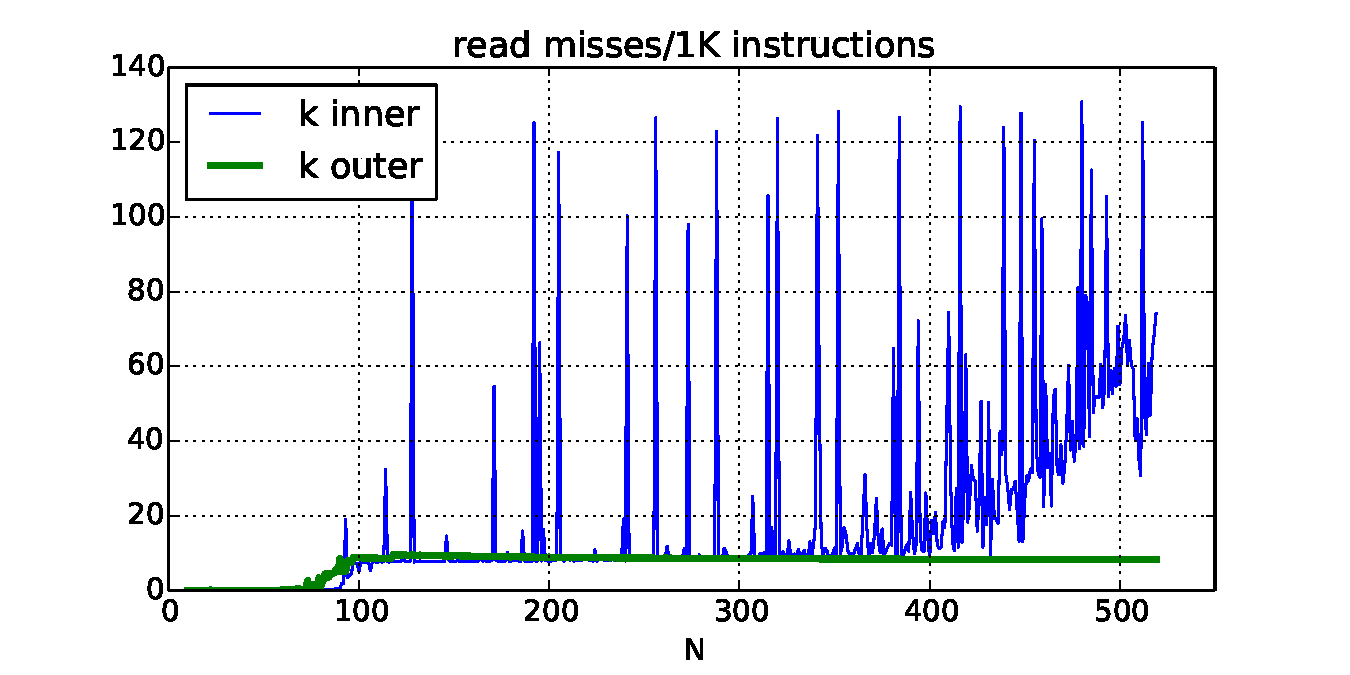
\includegraphics[width=0.99\textwidth]{../caching/k-inout-l1d_read_miss_rate}
\end{frame}

\begin{frame}{L1 miss detail (1)}
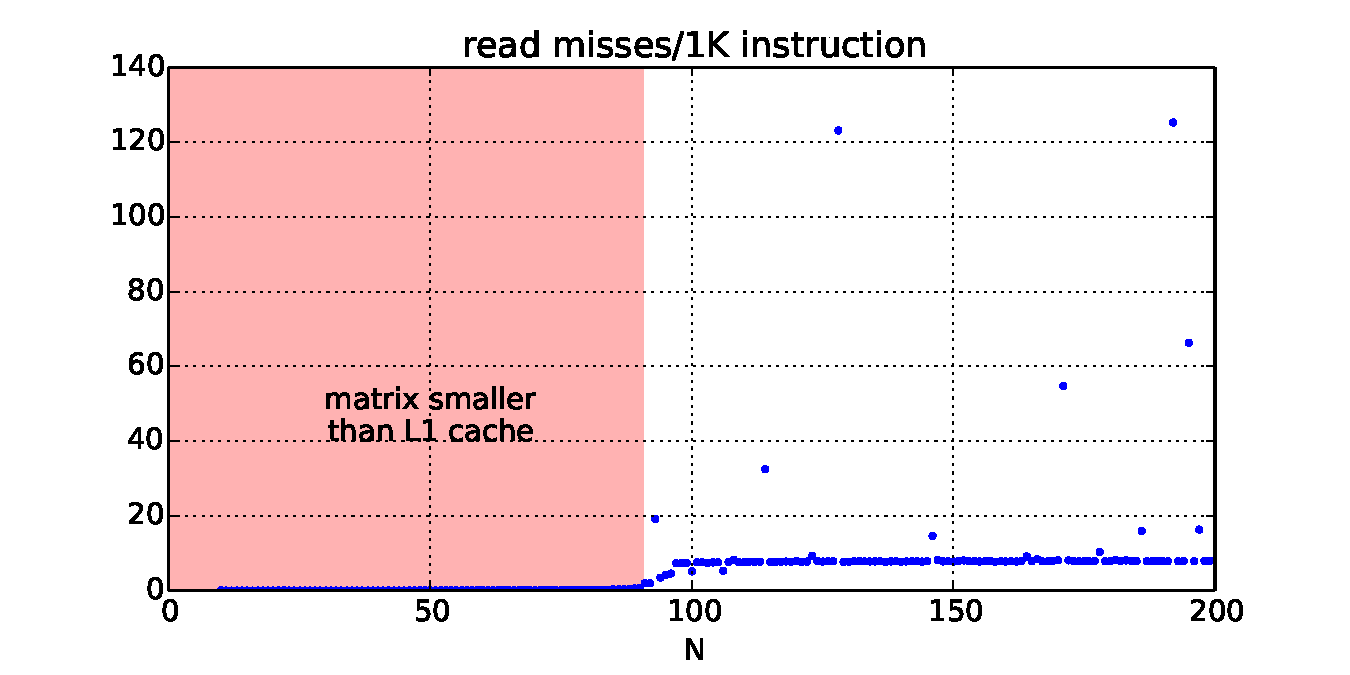
\includegraphics[width=0.99\textwidth]{../caching/k-in-l1d-miss-annot-size}
\end{frame}

\begin{frame}{L1 miss detail (2)}
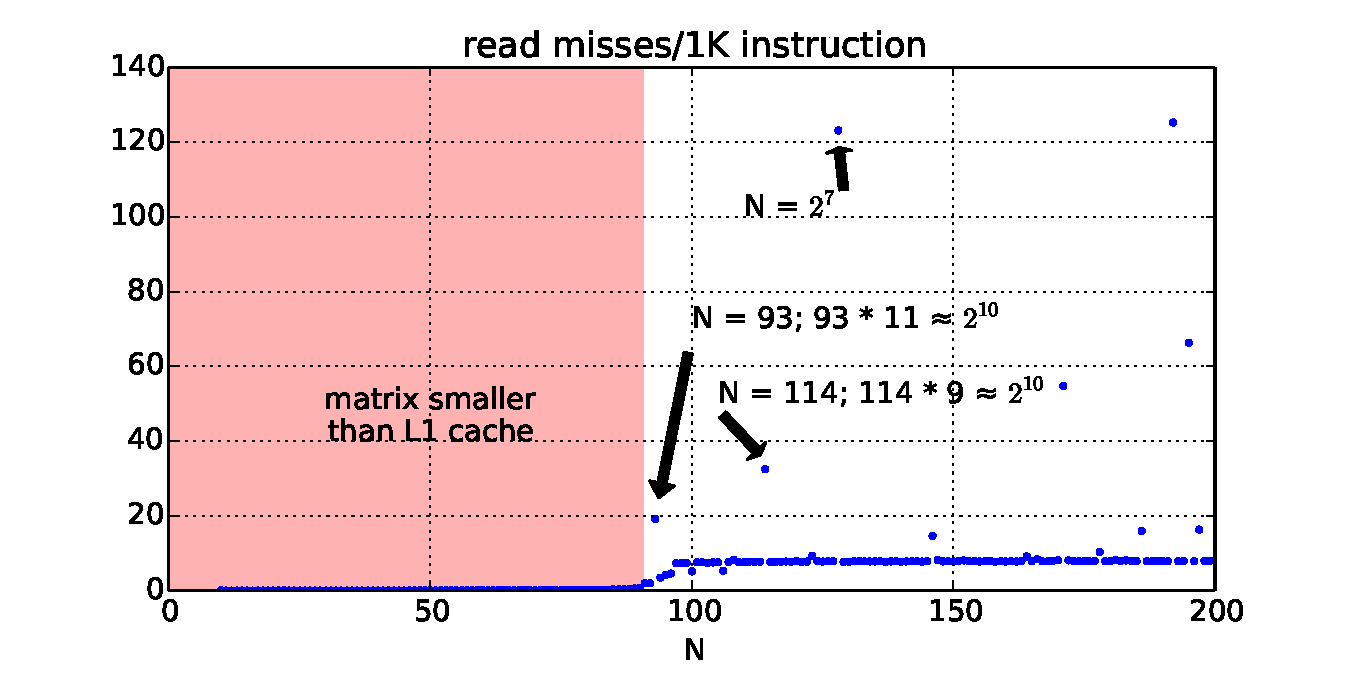
\includegraphics[width=0.99\textwidth]{../caching/k-in-l1d-miss-annot4-size}
\end{frame}

\begin{frame}[fragile,label=conflictExplainPre]{addresses}
    \begin{tabular}{lll}
        \lstinline|B[k*114+j]| &is at& \texttt{10 \textcolor<2>{blue!70!black}{\textbf<2>{0000 00}}00 0100} \\
        \lstinline|B[k*114+j+1]| &is at& \texttt{10 \textcolor<2>{blue!70!black}{\textbf<2>{0000 00}}00 1000} \\
        \lstinline|B[(k+1)*114+j]| &is at& \texttt{10 \textcolor<2>{blue!70!black}{\textbf<2>{0011 10}}01 0100} \\
        \lstinline|B[(k+2)*114+j]| &is at& \texttt{10 \textcolor<2>{blue!70!black}{\textbf<2>{0101 01}}01 1100} \\ 
        \ldots && \\
        \lstinline|B[(k+9)*114+j]| &is at& \texttt{11 \textcolor<2>{blue!70!black}{\textbf<2>{0000 00}}00 1100} \\
    \end{tabular}
    \vspace{.5cm}
    \begin{itemize}
\item<2> test system L1 cache: \textcolor<2>{blue!70!black}{6 index bits}, 6 block offset bits
\end{itemize}

\end{frame}


\begin{frame}[fragile,label=conflictExplain]{conflict misses}
\begin{itemize}
\item powers of two --- lower order bits unchanged
\item \lstinline|B[k*93+j]| and \lstinline|B[(k+11)*93+j]|:
    \begin{itemize}
        \item \myemph{1023 elements apart} (4092 bytes; 63.9 cache blocks)
    \end{itemize}
\item 64 sets in L1 cache: usually maps to same set
\item \lstinline|B[k*93+(j+1)]| will not be cached (next $i$ loop)
\item even if in same block as \lstinline|B[k*93+j]|
\vspace{.5cm}
\item how to fix? improve spatial locality
    \begin{itemize}
    \item (maybe even if it requires copying)
    \end{itemize}
\end{itemize}
\end{frame}
